\documentclass[11pt,a4paper]{article}

% ─── Packages ─────────────────────────────────────────

\usepackage{fontspec}
\setmainfont{Times New Roman}

\usepackage[top=1.0cm,bottom=0.9cm,left=1.45cm,right=1.45cm]{geometry}

\usepackage{titlesec}
\usepackage{enumitem}
\usepackage{hyperref}
\usepackage{xcolor}
\usepackage{tabularx}
\usepackage{graphicx}
\usepackage{parskip}

% ─── Colors ───────────────────────────────────────────

\definecolor{primary}{RGB}{30,40,90}
\definecolor{namecolor}{RGB}{0,120,180}
\definecolor{accent}{RGB}{50,90,150}
\definecolor{rulecol}{RGB}{200,205,220}
\definecolor{gray}{RGB}{90,90,90}

\hypersetup{
    colorlinks=true,
    urlcolor=accent
}

\pagestyle{empty}
\setlength{\parskip}{0pt}

% ─── Section ──────────────────────────────────────────

\titleformat{\section}
    {\normalsize\bfseries\color{primary}}
    {}
    {0em}
    {}
    [\vspace{1pt}\textcolor{rulecol}{\titlerule[0.6pt]}\vspace{1pt}]

\titlespacing{\section}{0pt}{4pt}{2pt}

% ─── Entry ────────────────────────────────────────────

\newcommand{\entry}[3]{%
    \noindent
    \begin{tabularx}{\linewidth}{X r}
        \textbf{\color{primary}#1} &
        {\scriptsize\color{gray}#2}
    \end{tabularx}\\[-2pt]
    {\scriptsize\textit{\color{gray}#3}}
    \vspace{0.5pt}
}

% ─── Compact list ─────────────────────────────────────

\newenvironment{cvitems}{
    \begin{itemize}[
        leftmargin=1.1em,
        topsep=0pt,
        itemsep=0.3pt,
        parsep=0pt,
        partopsep=0pt
    ]
}{
    \end{itemize}
}

% ═════════════════════════════════════════════════════

\begin{document}

% ─── HEADER ───────────────────────────────────────────

\noindent

\begin{tabularx}{\linewidth}{@{}X r@{}}

\begin{minipage}[c]{\linewidth}

    {\LARGE\bfseries\color{namecolor} Ho Huynh Nhu}\\[1pt]

    {\large\bfseries\color{primary}
    QA Staff}\\[2pt]

    {\scriptsize\color{gray}
    20/10/2003
    \enspace\textcolor{rulecol}{|}
    \enspace (+84) 367 503 477
    \enspace\textcolor{rulecol}{|}
    \enspace
    \href{mailto:hhnhu2003@gmail.com}{hhnhu2003@gmail.com}
    \enspace\textcolor{rulecol}{|}
    \enspace Ho Chi Minh City}\\[1pt]

    {\scriptsize
    \href{https://github.com/hohuynhnhu}
    {github.com/hohuynhnhu}
    \enspace\textcolor{rulecol}{|}
    \enspace
    \href{https://www.facebook.com/huynhnhu.ho.961}
    {facebook.com/huynhnhu.ho.961}
    }

\end{minipage}

&

\begin{minipage}[c]{2.1cm}
    \raggedleft
    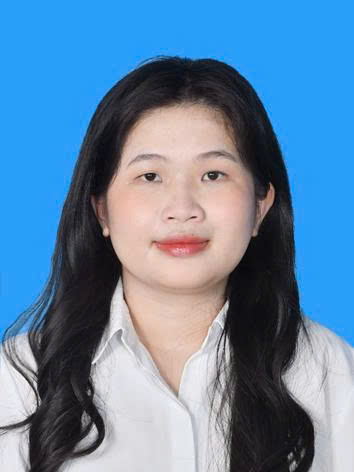
\includegraphics[
        width=2.1cm,
        height=2.5cm,
        keepaspectratio
    ]{assets/avt.jpg}
\end{minipage}

\end{tabularx}

\vspace{2pt}

\textcolor{rulecol}{\rule{\linewidth}{0.6pt}}

% ─── CAREER OBJECTIVE ─────────────────────────────────

\section*{Career Objective}

{\small
Final-year Information Technology student seeking a QA position, with a basic understanding of software testing and hands-on experience in SQL, Python, API testing using Postman, and Jira. Detail-oriented and logical, with experience validating data, identifying errors, and reporting results clearly. Eager to learn software testing processes, improve testing skills, and contribute to delivering reliable software products.
}

% ─── EDUCATION ────────────────────────────────────────

\section*{Education}

\entry
{University of Transport Ho Chi Minh City (UTH)}
{10/2022 -- 10/2026}
{Bachelor of Information Technology -- Completed coursework}

{\small
\begin{cvitems}

    \item GPA: \textbf{3.4 / 4.0}

    \item \textbf{Excellent Scholarship} -- Semester 1, 2025

    \item \textbf{Second Prize -- AI Track},
    UTH Student Scientific Research Conference 2025

\end{cvitems}
}

% ─── TECHNICAL SKILLS ─────────────────────────────────

\section*{Technical Skills}

{\small

\begin{tabularx}{\linewidth}{@{}lX@{}}


\textbf{Software Testing}
&
Manual Testing (Web/Mobile), Test Case \& Test Checklist, Bug/Defect Reporting,
Data Validation
\\[1pt]

\textbf{Bug Tracking \& Collaboration}
&
Jira, Confluence, Git, Daily/Weekly Progress Reporting
\\[1pt]

\textbf{API / Database}
&
Postman, RESTful API, SQL, PostgreSQL, SQL Server, MySQL,
Joins, Aggregations, MongoDB, Firebase
\\[1pt]

\textbf{Generative AI}
&
LLMs, Retrieval-Augmented Generation (RAG), AI-assisted Analysis
\\[1pt]

\textbf{Programming}
&
Python, Pandas, NumPy, FastAPI, TypeScript, JavaScript, Kotlin
\\[1pt]

\textbf{Data / BI}
&
Power BI, Excel, ETL/ELT, dbt, Apache Airflow, Docker
\\[1pt]
\textbf{English}
&
TOEIC 500; reading technical documents, writing bug reports and basic communication


\end{tabularx}

}

% ─── WORK EXPERIENCE ──────────────────────────────────

\section*{Work Experience}

\entry
{Gotik Consulting -- Data Engineer}
{Python \textbar{} dbt \textbar{} PostgreSQL \textbar{} Airflow \textbar{} Power BI}
{03/2026 -- 05/2026}

{\small
\begin{cvitems}
    \item Wrote SQL queries to aggregate, filter, and join data, and cross-checked results to ensure reliable data sources for dashboards and reports.

    \item Cleaned and validated Odoo business data with Python and SQL to detect inconsistencies and prepare accurate, structured datasets.

    \item Monitored scheduled Airflow workflows (hourly ETL runs), tracking task dependencies and failures to keep data pipelines stable.

    \item Developed dbt models to standardize raw data, improving data consistency and making results easier to verify and reuse.

    \item Built Power BI dashboards and regular reports on operational metrics for monitoring and review.
\end{cvitems}
}

% ─── PROJECTS ─────────────────────────────────────────

\section*{Featured Projects}

\entry
{Fall Detection -- Machine Learning Classification System}
{Python \textbar{} PyTorch \textbar{} YOLOv8 Pose \textbar{} MediaPipe \textbar{} Transformer}
{04/2026 -- 06/2026}

{\small
\begin{cvitems}

    \item Prepared video datasets and extracted human pose features
    using MediaPipe and YOLOv8 Pose for fall/non-fall classification.

    \item Developed and trained a Transformer Encoder for binary
    classification using sequential pose features.

    \item Achieved 97.8\% mean accuracy with 5-fold cross-validation
    and evaluated model performance on unseen data.

\end{cvitems}
}

\vspace{3pt}

\entry
{VehicleScan -- AI-Based Vehicle Recognition System}
{Python \textbar{} YOLO \textbar{} CNN \textbar{} Siamese Network \textbar{} Firebase}
{03/2025 -- 03/2026}

{\small
\begin{cvitems}

    \item Prepared and labeled datasets for vehicle detection,
    classification, and recognition tasks.

    \item Trained and evaluated YOLO, CNN, and Siamese Network models
    for vehicle identification and recognition.

    \item Applied image preprocessing and feature extraction, and
    achieved Second Prize -- AI Track at UTH 2025.

\end{cvitems}
}

% % ─── ADDITIONAL INFORMATION ───────────────────────────

% \section*{Additional Information}

% {\small

% \begin{tabularx}{\linewidth}{@{}lX@{}}

% \textbf{Soft Skills}
% &
% Careful and detail-oriented \textbar{} Logical thinking \textbar{}
% Responsible \textbar{} Clear reporting \textbar{} Teamwork

% \\[1pt]

% \textbf{Availability}
% &
% Available for full-time QA Engineer opportunities.

% \end{tabularx}

% }
\end{document}